\chapter{Discussion, Conclusion and Future Work}\label{chapter:discussion}

In this chapter, we discuss the results of the experiments conducted in Chapter \ref{chapter:results}. We will discuss the effect of different parameters on the performance of the models, 
and how they relate to the original goals of this thesis. We then conclude with a summary of the findings and suggest future work that can be done.

\section{Effect of Phoneme Count}

\begin{figure}[H]  
    \centering
    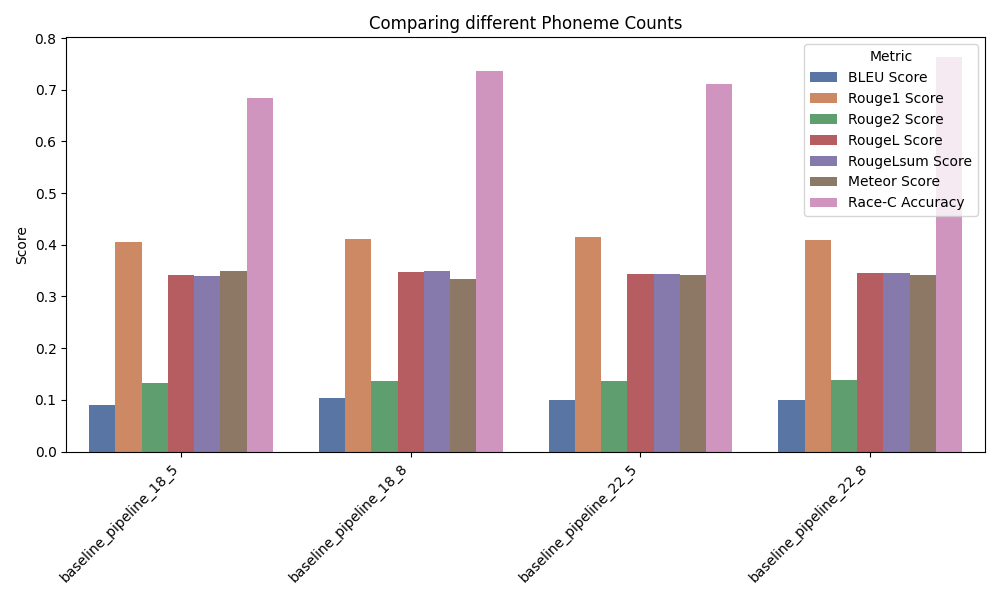
\includegraphics[width=0.7\linewidth]{figures/results/1_effect_of_phoneme_count.png}
    \caption{Comparing the Effects of different phoneme counts}
    \label{fig:compare-phoneme-count}
\end{figure}

As we can see in Figure \ref{fig:compare-phoneme-count}, the phoneme count does not seem to have a significant effect on the translation scores
or the Race-C scores. This being the case, we can conclude that we can simplify a language by reducing the phoneme count without affecting the 
ability of the language to convey meaning. 

\section{Effect of Phonotactics}

\begin{figure}[H]  
    \centering
    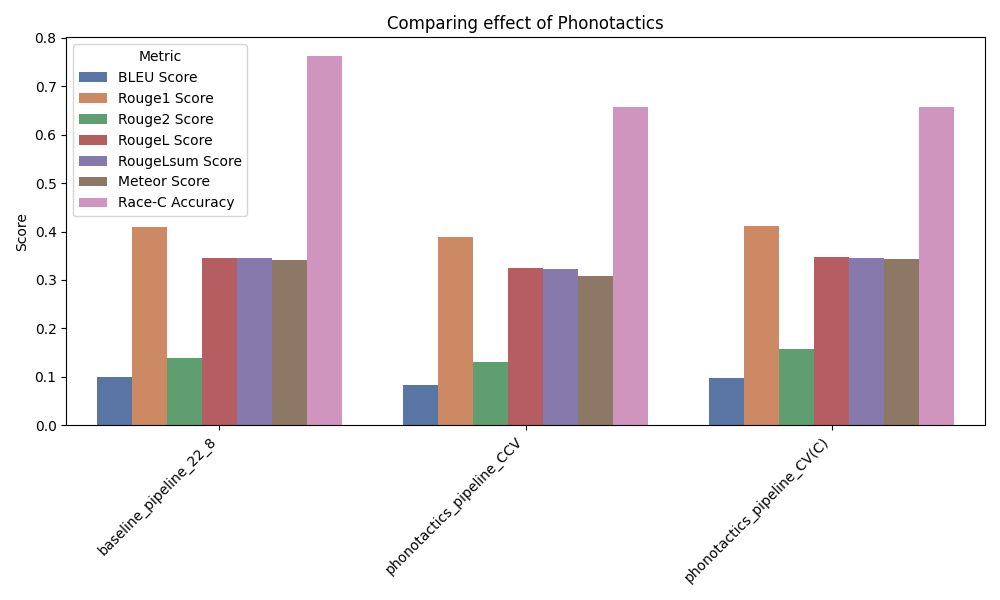
\includegraphics[width=0.7\linewidth]{figures/results/1_effect_of_phonotactics.png}
    \caption{Comparing the Effects of phonotactics}
    \label{fig:compare-phonotactics}
\end{figure}

Figure \ref{fig:compare-phonotactics} shows the effect of phonotactics on the translation scores and the Race-C scores. Again, we can see that
the phonotactics do not seem to have a significant effect either of the metrics. We can therefore conclude that we can simplify a language by 
using simplifed phonotactic rules without affecting the ability of the language to convey meaning.

\section{Effect of Grammar Rules}

\begin{figure}[H]  
    \centering
    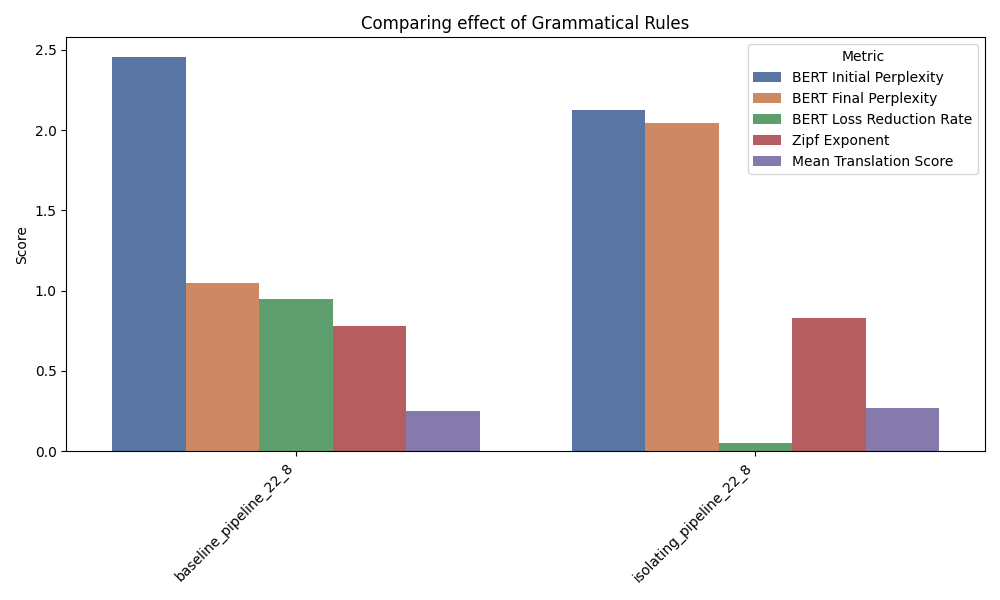
\includegraphics[width=0.7\linewidth]{figures/results/1_effect_of_grammar.png}
    \caption{Comparing different Grammatical Rules}
    \label{fig:compare-grammar}
\end{figure}

We implemented 2 different grammars, but from our results we did not find any significant difference between the Agglutinative and Isolating 
grammar modules, save for differences in the Final Perplexity in the Bert Evaluation. Further investigation is required to analyse the effects
of grammatical features in constructed languages.

\section{Effect of Vocabulary Generation method}

Figure \ref{fig:compare-vocab-gen-types} shows the effect of different simplifying vocabulary generation methods against our metrics.
We can see that both methods result in a drop in the translation scores, and in the Race-C scores. We can consider the ratio of the Mean Translation Score (MTS) and 
the Race-C Accuracy to the vocabulary size.

\begin{figure}[H]
    \centering
    \begin{subfigure}[b]{0.48\linewidth}
        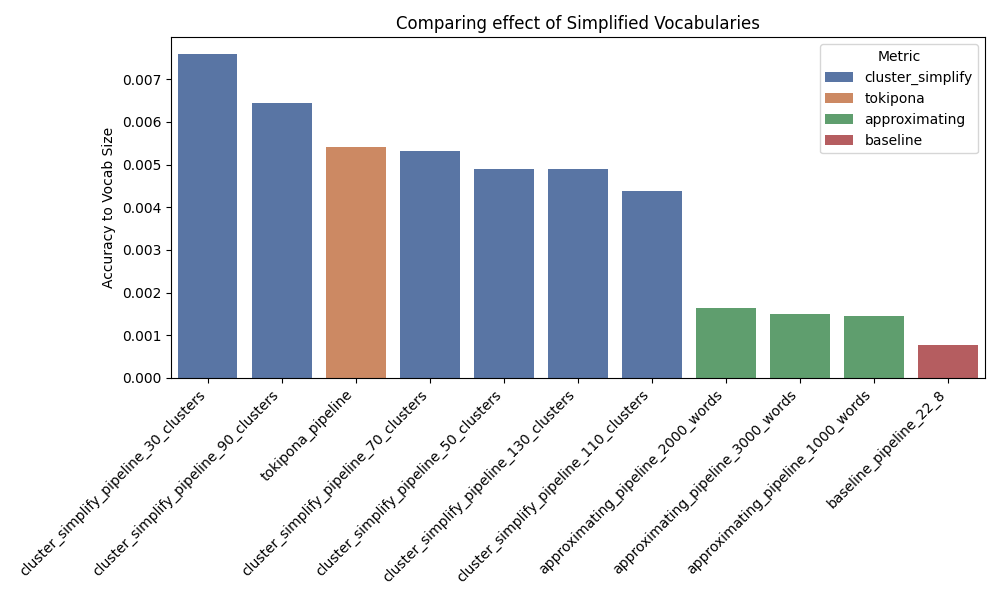
\includegraphics[width=\linewidth]{figures/results/1_effect_of_vocab_simplify.png}
        \caption{Effect of Vocabulary on Race-C Accuracy}
        \label{fig:vocabulary-effect-rc}
    \end{subfigure}
    \hfill
    \begin{subfigure}[b]{0.48\textwidth}
        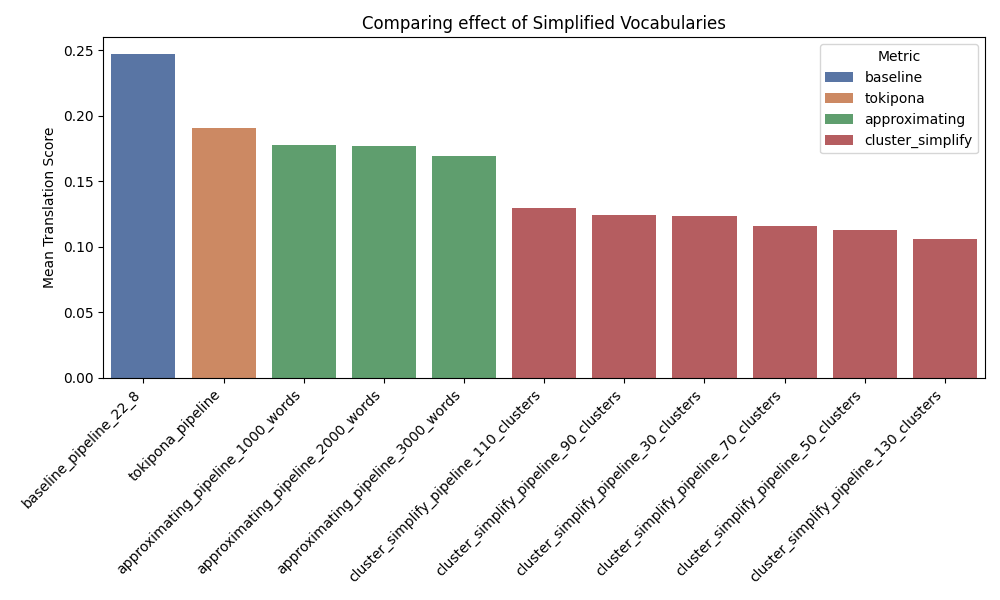
\includegraphics[width=\linewidth]{figures/results/1_effect_of_vocab_simplify_mts.png}
        \caption{Effect of Vocabulary on MTS}
        \label{fig:vocabulary-effect-mts}
    \end{subfigure}
    \caption{Effect of Simplified Vocabulary.}
    \label{fig:vocabulary-effect-mts-rc}
\end{figure}

From Figure \ref{fig:vocabulary-effect-mts}, we can see that the drop in MTS Score is much more significant, with the baseline having the highest ratio. However,
as we can see from Figure \ref{fig:vocabulary-effect-rc}, The cluster-simplify and approximating methods perform better in terms of accuracy to vocabulary size.
For all practical purposes, we can argue that the performance on the Reading Comprehension dataset is a better proxy for the performance of the language, rather than the MTS scores,
which heavily depend on n-gram similarity.

\section{Effect of Language Model Temperature}
We compared the effects of different model temperatures on the evaluations, with the same baseline pipeline. The baseline was run with a temperature value of 
\texttt{0.2}. From Figure \ref{fig:compare-temperature}, we can see that the higher model temperature seems to degrade the result of some scores, but 
does not seem to have a significant effect with a lower temperature. We can conclude that the results can be reproduced at different model temperatures, as long as 
the temperature is not too high. 
\begin{figure}[H]  
    \centering
    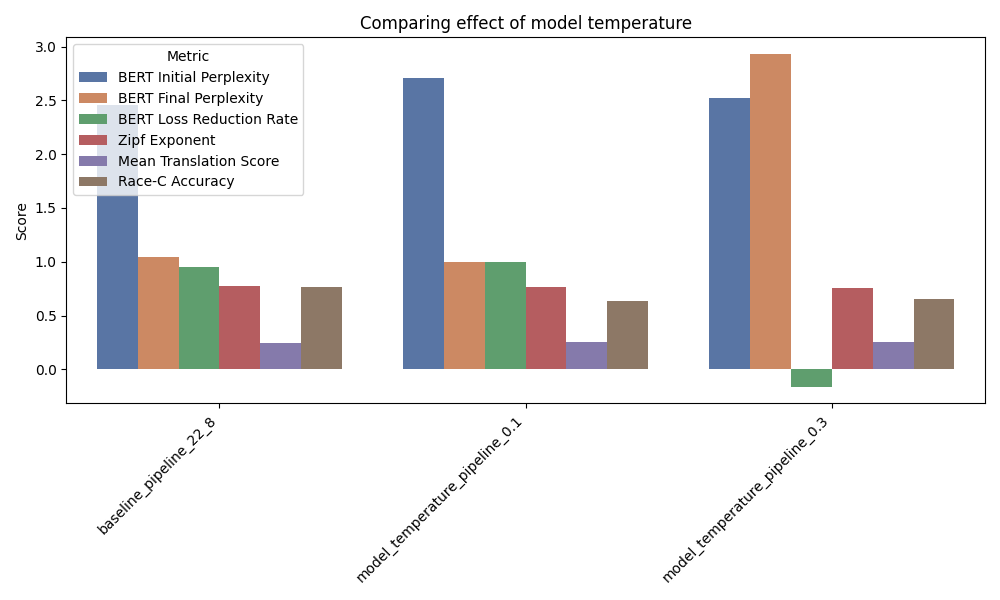
\includegraphics[width=0.7\linewidth]{figures/results/1_effect_of_model_temperature.png}
    \caption{Effect of Model Temperature}
    \label{fig:compare-temperature}
\end{figure}


\section{Conclusion}
This thesis set out to investigate whether pre-trained Large Language Models (LLMs) can aid in the systematic construction of minimal, efficient 
languages that preserve communicative utility. By developing a modular pipeline that integrates phonology, phonotactics, grammar, vocabulary, and multiple evaluation strategies, 
we were able to design and assess a variety of constructed languages (ConLangs) under different constraints.

The results demonstrate that significant simplifications are possible in multiple linguistic subsystems, such as reducing phoneme inventory and grammar complexity,
without substantially degrading performance on machine translation or comprehension tasks. In particular, reading comprehension scores remained relatively robust even in highly 
simplified setups, indicating that core meaning can be preserved despite a reduction in language complexity. Additionally, the adherence to Zipf's Law in many generated languages 
suggests that even artificial languages can naturally align with linguistic patterns found in human languages.

Our experiments show that LLMs can effectively support language generation and evaluation, acting as tools to explore the trade-off between efficiency and expressiveness in language design. 
The modularity of our framework allows for targeted ablation studies, making it a flexible foundation for future research in computational linguistics and language optimization.

In essence, this work provides strong evidence that LLMs can assist in creating interpretable, compact, and efficient constructed languages, 
opening new avenues for both linguistic theory and applied language technology.


\section{Future Work}
The results of this thesis show that it is possible to generate simplified languages that are still able to convey meaning. However, there are still many
open areas for future work. Firstly, we can explore other different language generation methods, including more or less complex grammatical rules,
or different vocabulary generation methods. In particular, further research is required in analyzing the effects of different grammatical structures.

In addition, further research is required on metrics to evaluate the generated languages. In particular, there is more to explore
in terms of simplicity measures, which are complex to define and measure.
